\documentclass{article}

% ------------------------------------ %
%             Document Info            %
% ------------------------------------ %

\usepackage{../../../LaTeX-Preamables/Assign}

\begin{document}
\newcommand{\documentcourse}{ENGG1300}
\newcommand{\documentnumber}{2}

% ------------------------------------ %
%                Header                %
% ------------------------------------ %

\begin{minipage}{0.07\textwidth}
    
\includegraphics[width=\linewidth]{../../../LaTeX-Preamables/LaTeX-Templates/HKULOGO256.png}
\end{minipage}
\hspace{0.02\textwidth}
\begin{minipage}{0.55\textwidth}
    \documentcourse

    Assignment \documentnumber

    SID: 3036268218
\end{minipage}
\begin{minipage}{0.35\textwidth}
    \begin{flushright}
        Jax

        \jobname.pdf

        \today
    \end{flushright}
\end{minipage}

\vspace{0.5cm}

\hrule

% ------------------------------------ %
%                Content               %
% ------------------------------------ %

\section*{Question 6}
\begin{center}
    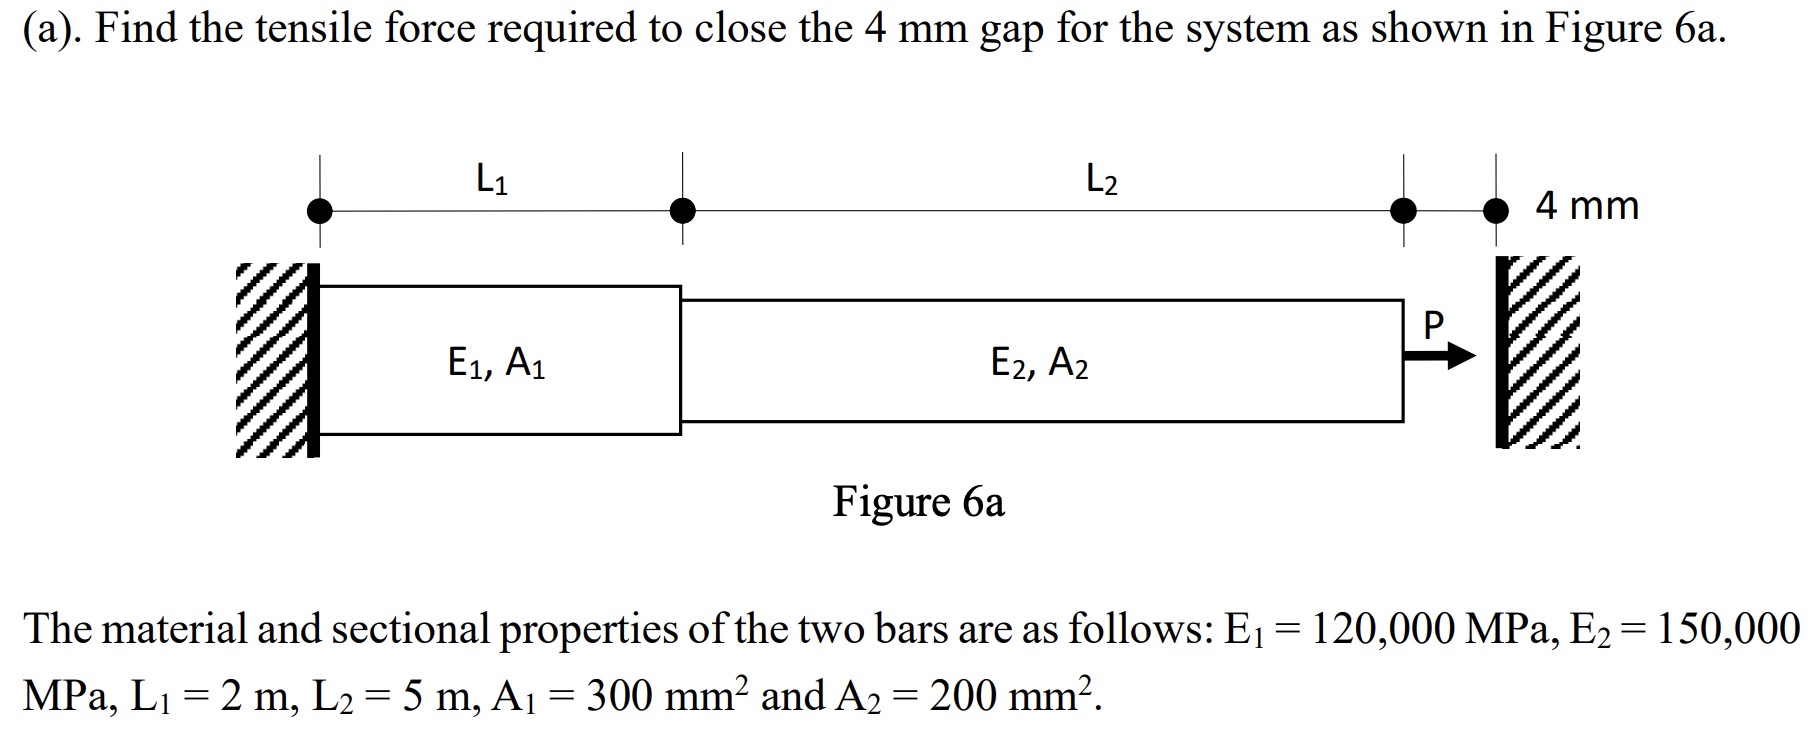
\includegraphics[width=0.8\textwidth]{img/2-1.jpg}
\end{center}
\begin{align*}
    E                                                                                                & =\frac{Fx}{A\Delta x} \\
    \Delta x                                                                                         & = \frac{Fx}{AE}       \\
    \Delta x_1 + \Delta x_2                                                                          & = 4mm                 \\
    \frac{P\times 2}{0.0003\times 120000\times 10^6}+\frac{P\times 5}{0.0002\times 150000\times10^6} & =0.004                \\
    P                                                                                                & = 18kN
\end{align*}

\begin{center}
    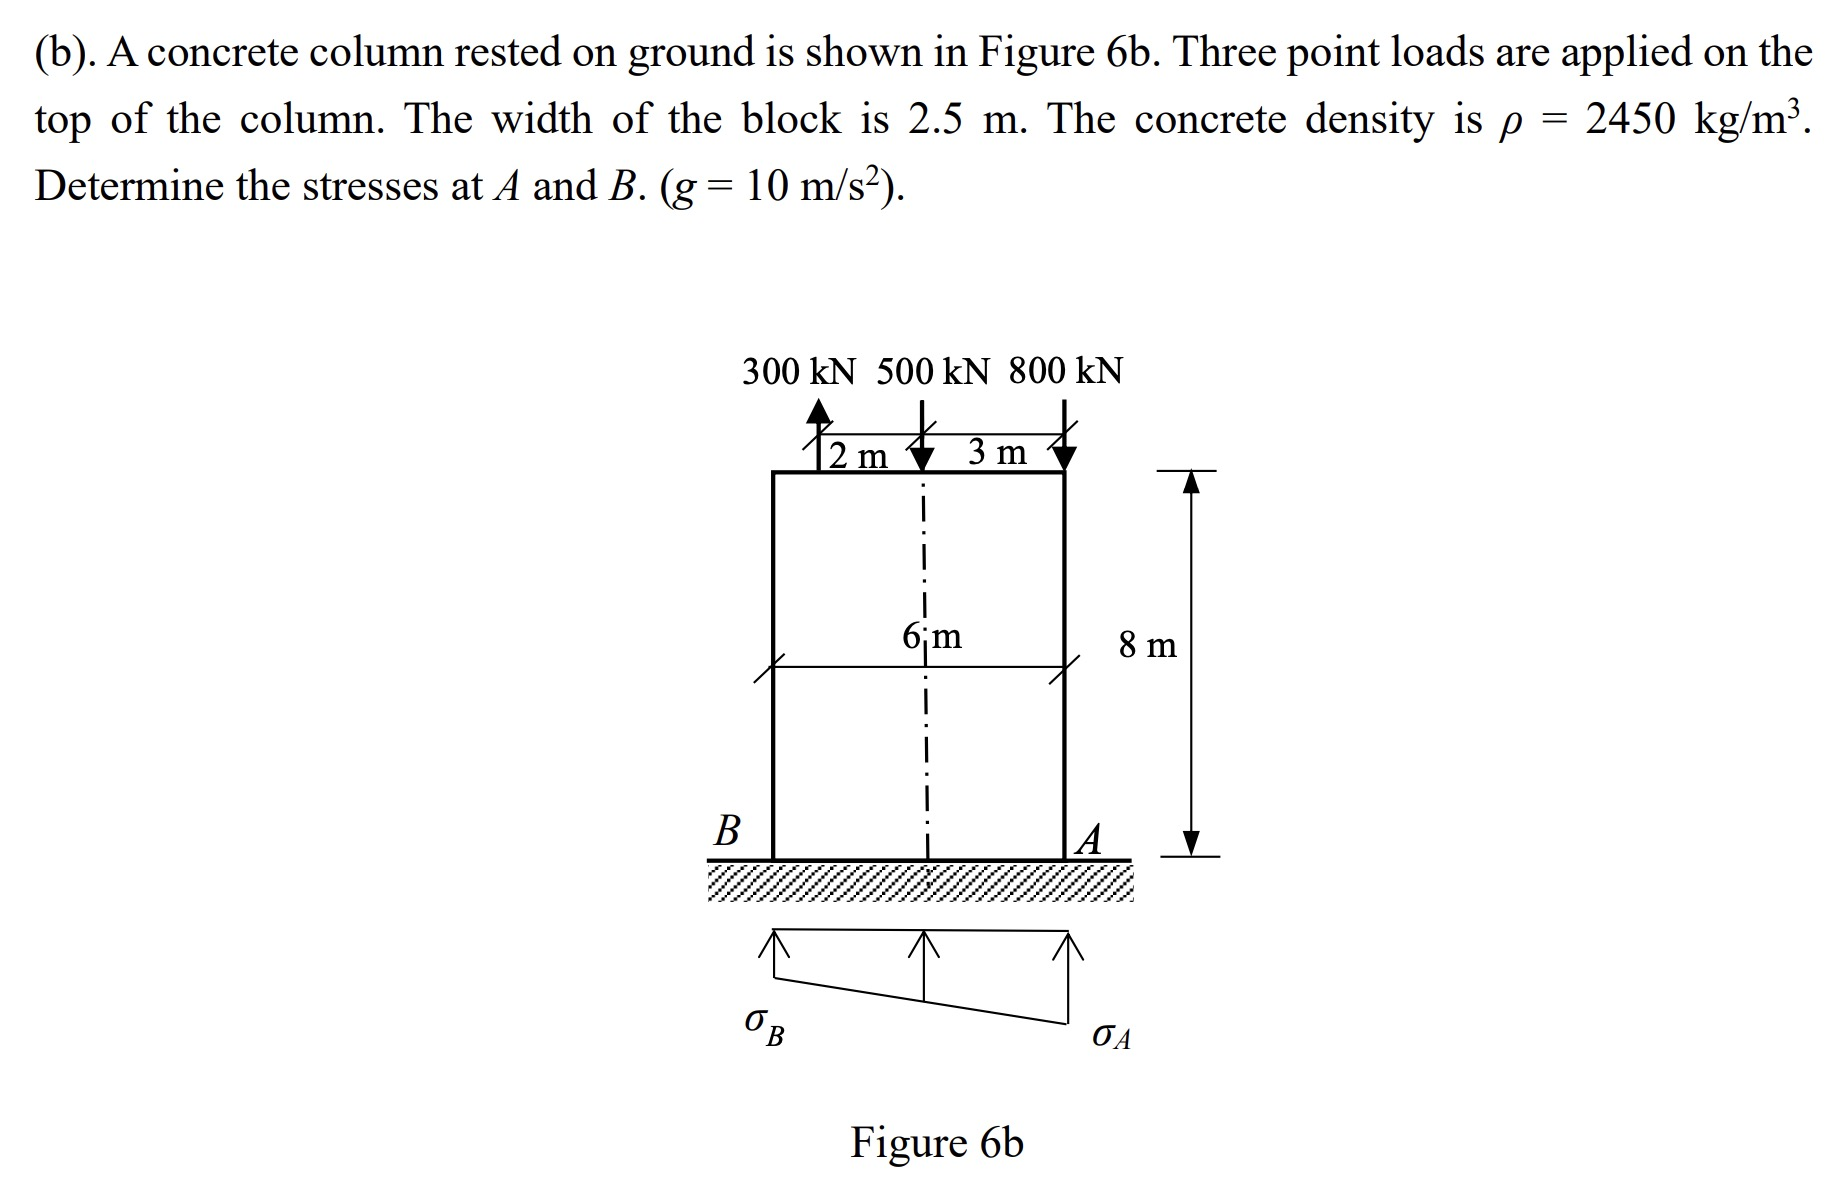
\includegraphics[width=0.8\textwidth]{img/2-2.jpg}
\end{center}
Consider units in kN:
\begin{align*}
    \sigma_{axial} = \frac{(500 + 800 - 300)+\frac{2450\times6\times8\times2.5\times10}{1000}}{6\times2.5} & = 262.667                                                  \\
    \sigma_{flex}                                                                                          & =\frac{6\times800\times3+6\times300\times2}{2.5\times 6^2} \\
                                                                                                           & = 200\ Pa                                                  \\
    \sigma_B = \sigma_{axial} - 200                                                                        & = 62.67\ Pa                                                \\
    \sigma_A = \sigma_{axial} + 200                                                                        & = 462.67\ Pa                                               \\
\end{align*}
% TODO: ADD TO NOTES

\section*{Question 7}
\begin{center}
    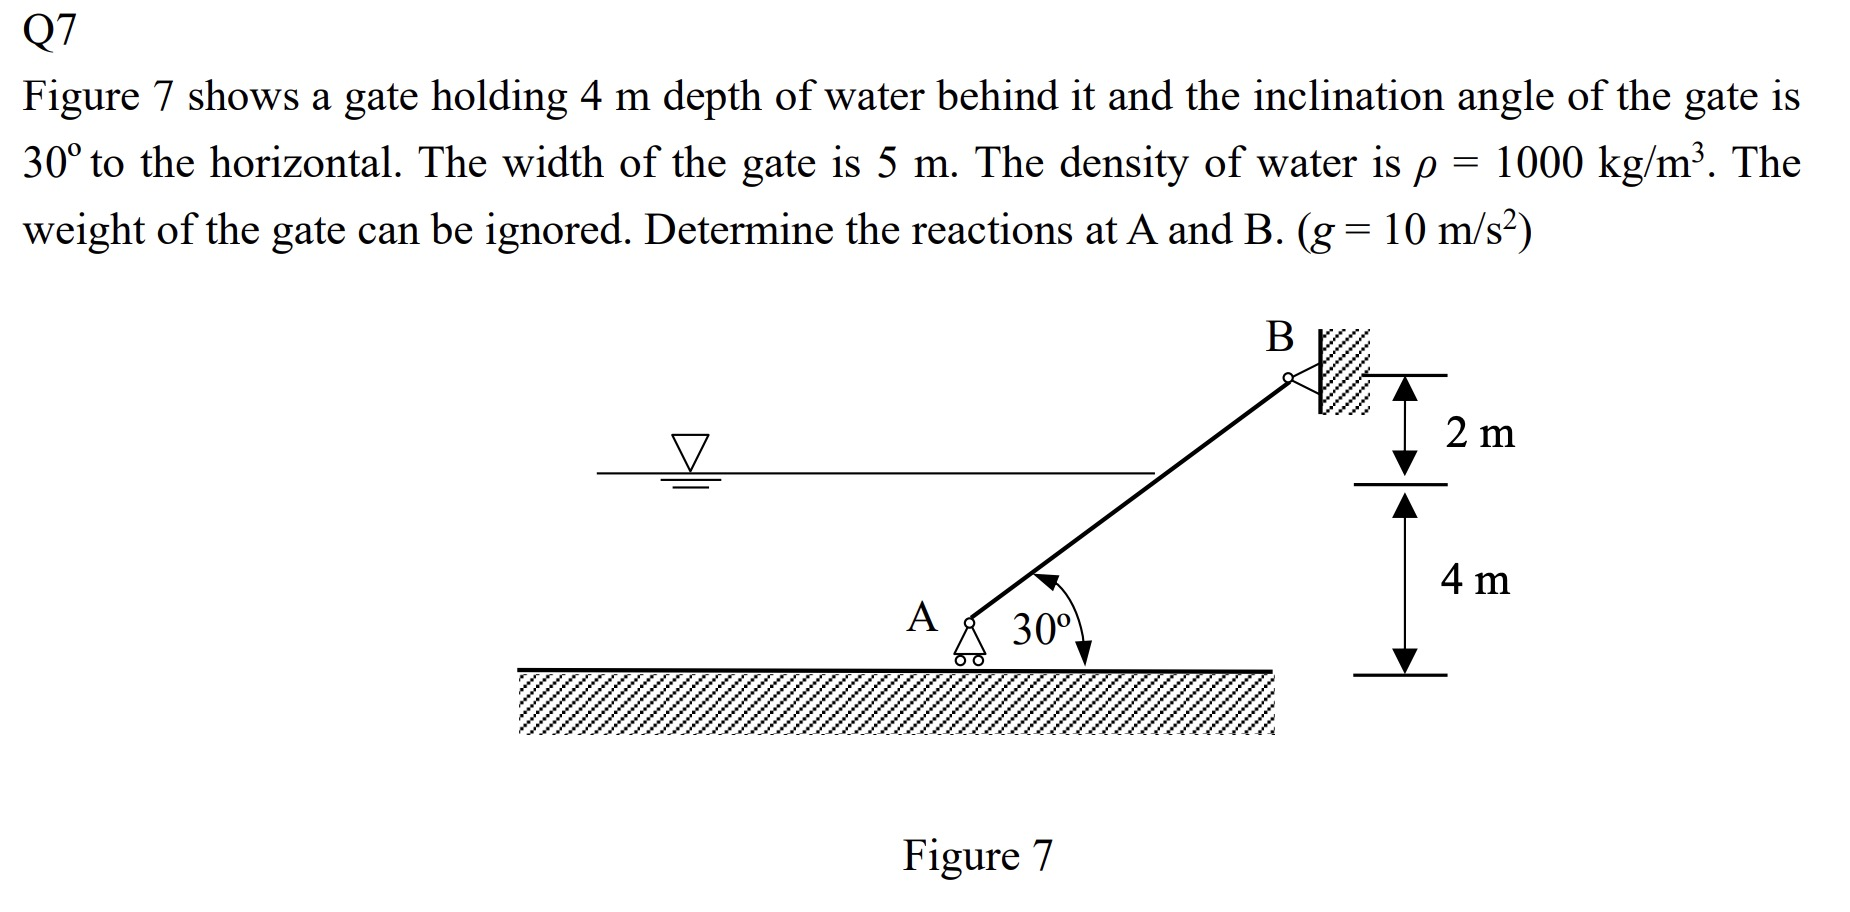
\includegraphics[width=0.8\textwidth]{img/2-3.jpg}
\end{center}
The force exerted onto the gate by the water pressure is:
\begin{align*}
    F_p & =\frac{\rho g d w L}{2}                                        \\
        & = \frac{1000\cdot10\cdot4\cdot5\cdot\frac{4}{\sin30^\circ}}{2} \\
        & = 800\ kN
\end{align*}
$F_R$ is located at $\frac{8}{3}$ from the base.
\begin{align*}
    L                               & = 12m                               \\
    \\
    \sum M_B                        & = 0                                 \\
    F_p\times(\frac{8\times2}{3}+4) & = F_{A}\sin(60^\circ)\times12       \\
    F_{A}                           & =718.48\ kN\text{ up}               \\
    \\
    \sum F_{x}                      & =0                                  \\
    F_{Bx}                          & = F_p \times \cos(60^\circ)         \\
                                    & = 400\ kN\text{ to the left}        \\
    \sum F_{y}                      & = 0                                 \\
    F_{By}                          & = F_p \times \sin(60^\circ) - F_{A} \\
                                    & = 25.66\ kN\text{ downward}         \\
\end{align*}

\section*{Question 8}
\begin{center}
    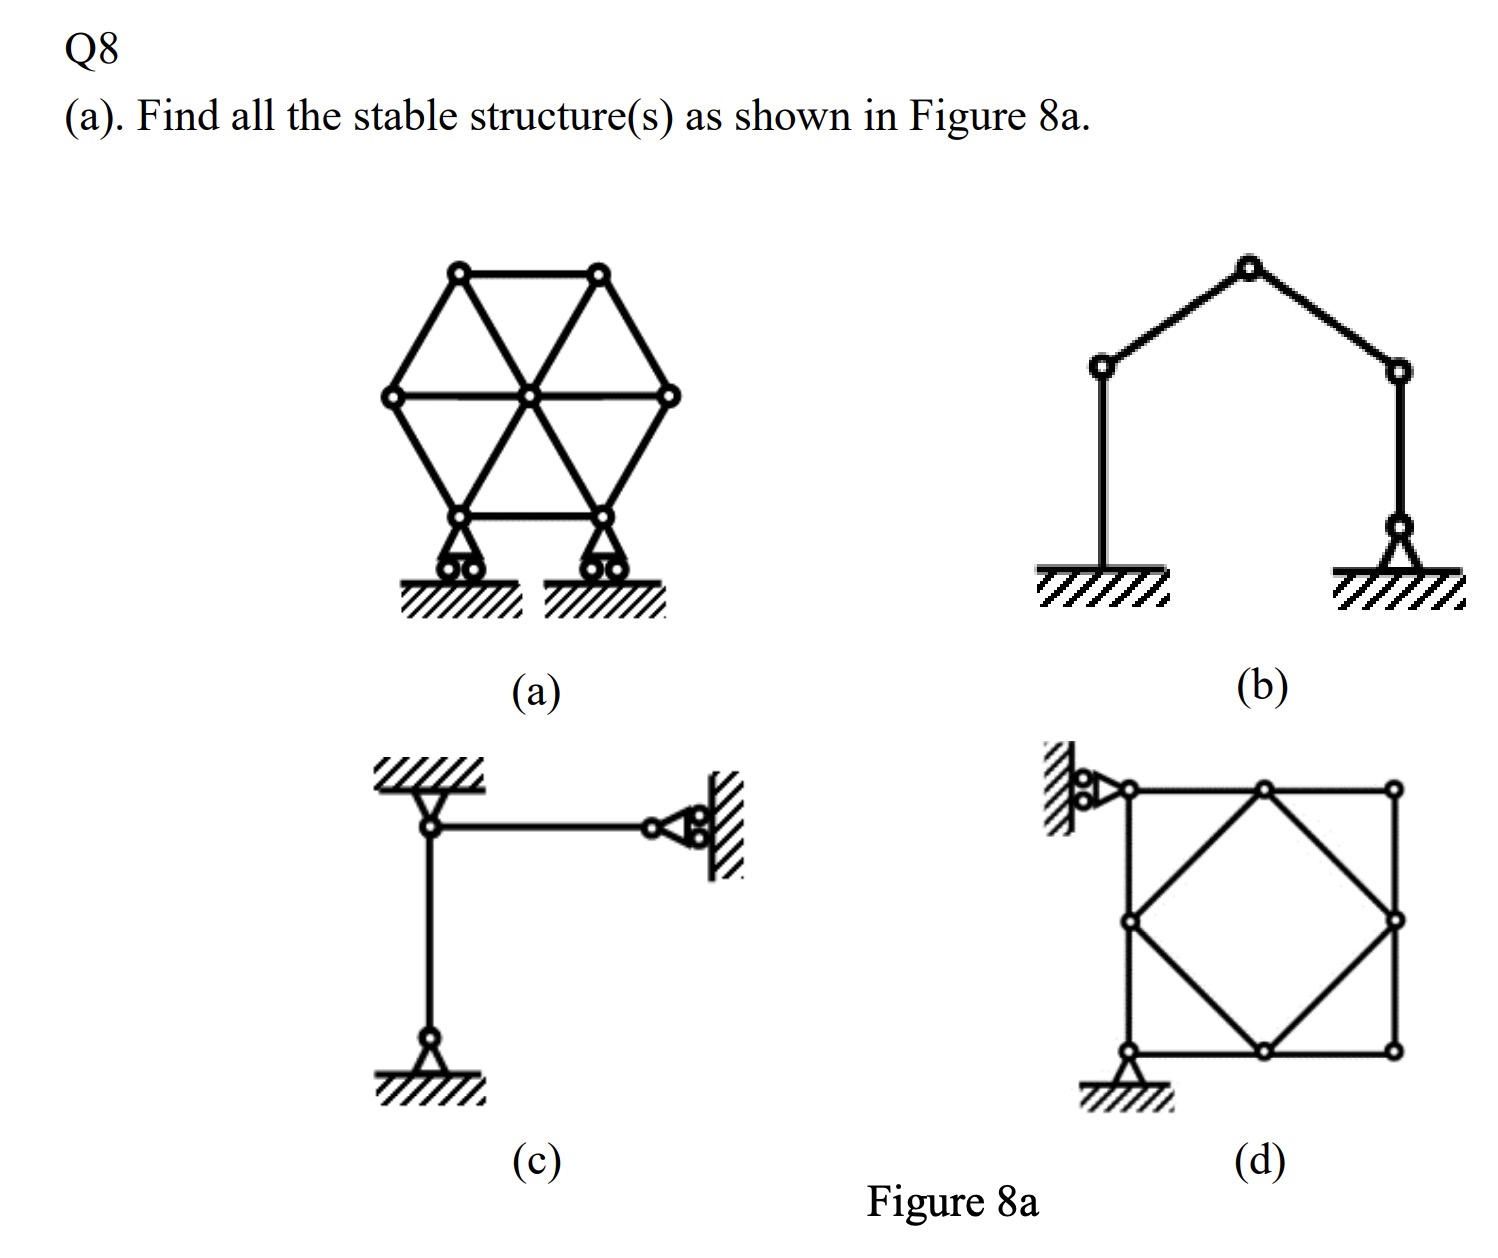
\includegraphics[width=0.5\textwidth]{img/2-4.jpg}
\end{center}
There are no stable structures.

\begin{center}
    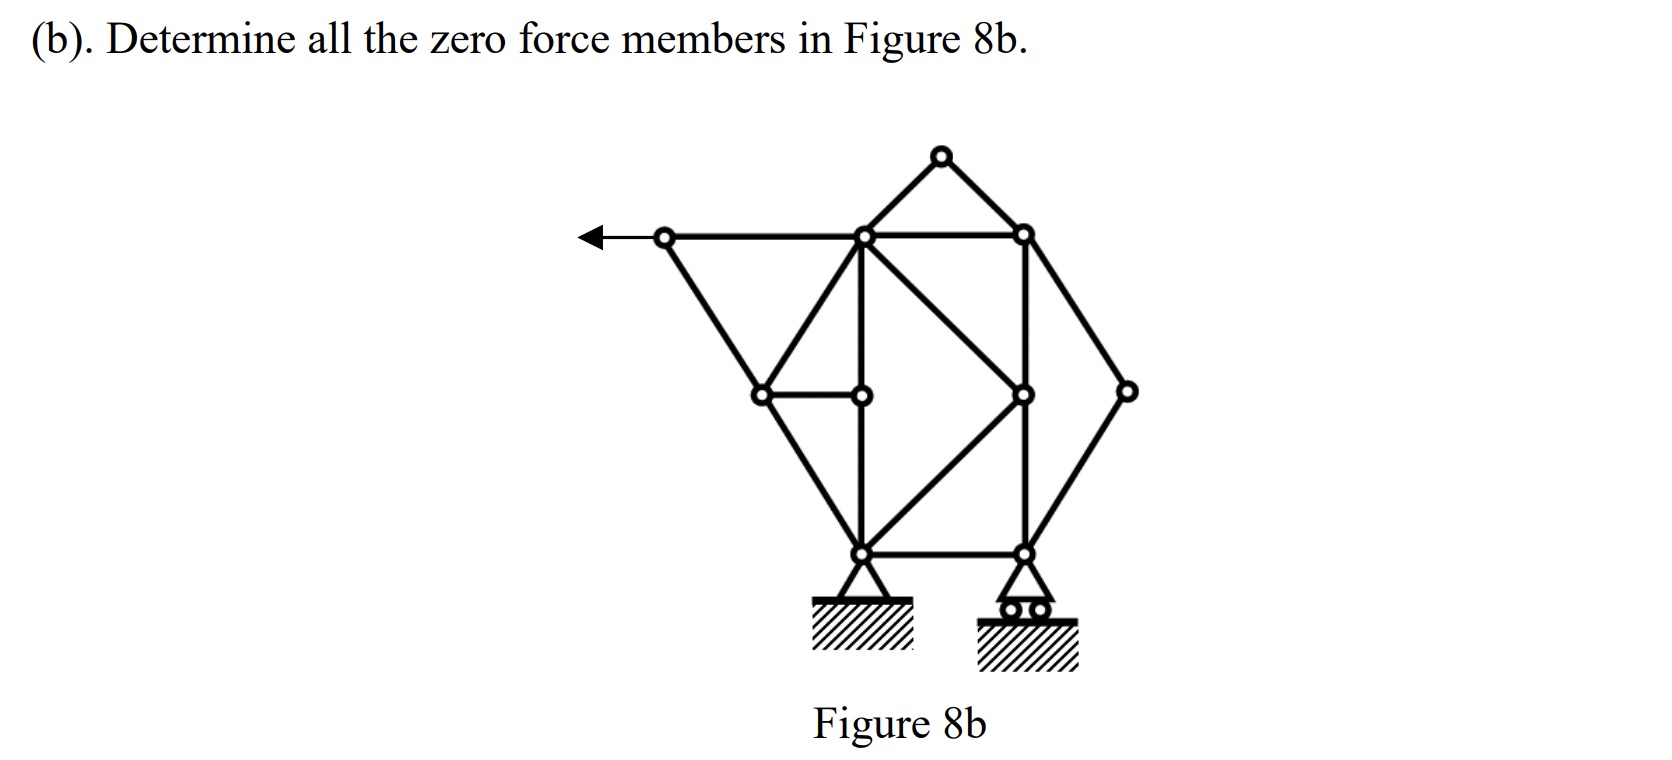
\includegraphics[width=0.5\textwidth]{img/2-5.jpg}

\end{center}
Highlighted all zero-force members.

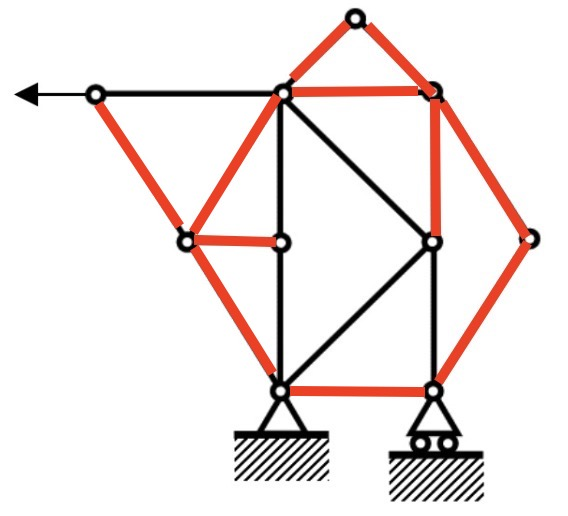
\includegraphics[width=0.2\textwidth]{img/2-8b.jpg}

\begin{center}
    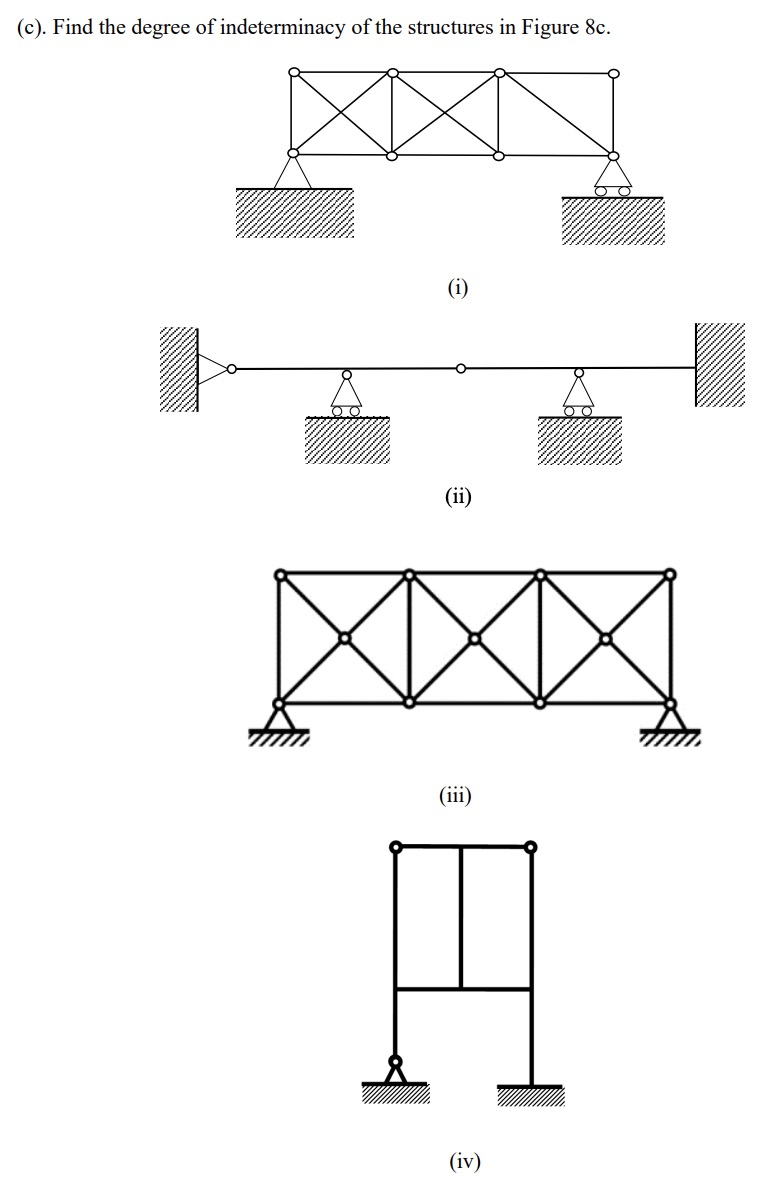
\includegraphics[width=0.5\textwidth]{img/2-6.jpg}
\end{center}

i: Reaction (r) = 3, joints (j) = 8, members (m) = 15, $(r+m)>2j\to 18>16$, Indeterminancy is 2\\
ii: r = 7, j = 4, m = 4, $(r+m)>2j\to 11>8$, Indeterminancy is 3\\
iii: r = 4, j = 11, m = 22, $(r+m)>2j\to 26>22$, Indeterminancy is 4\\
iv: Indeterminancy is 3+3+2 = 8\\

% FIXME:
\section*{Question 9}
\begin{center}
    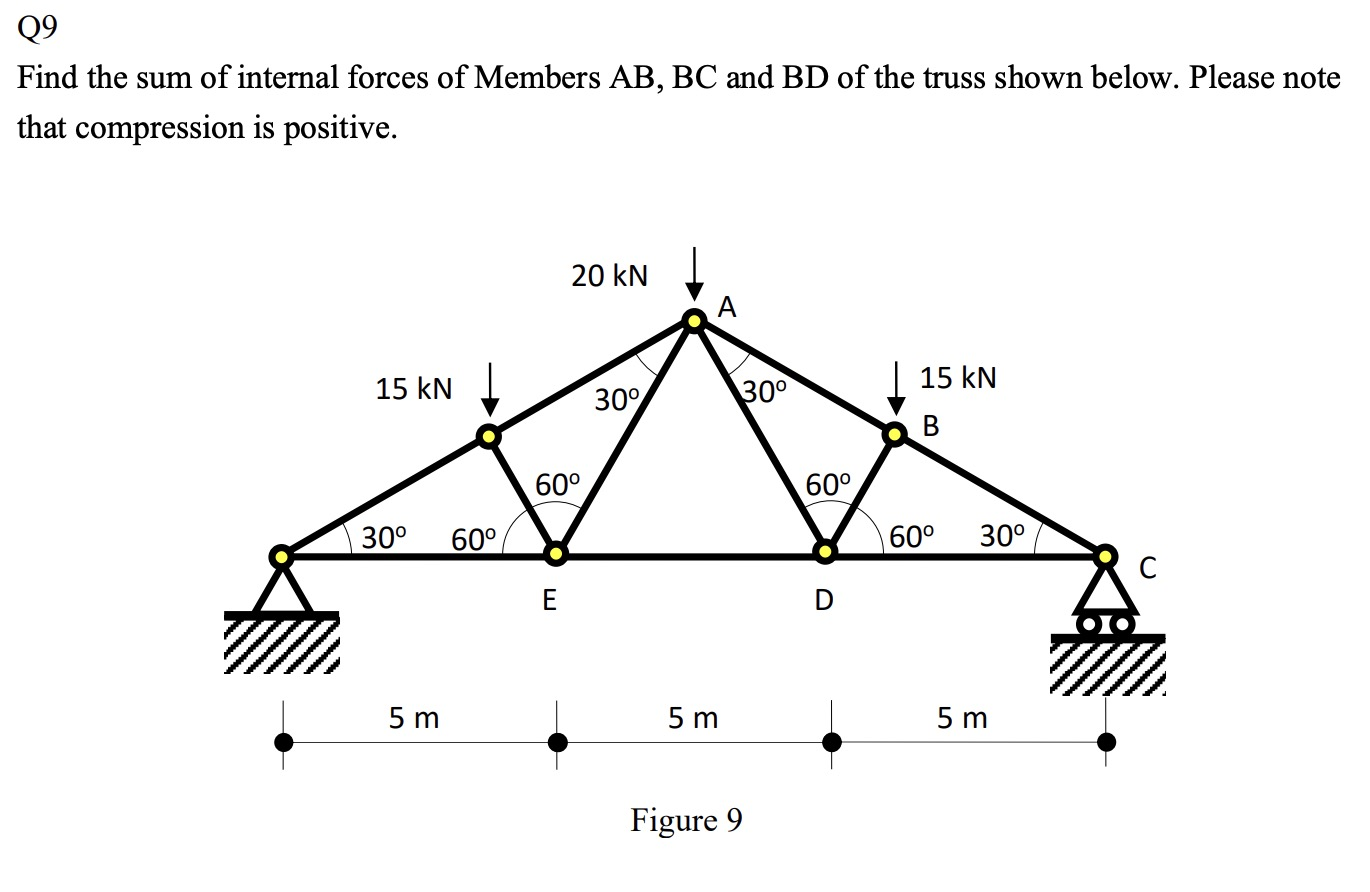
\includegraphics[width=0.5\textwidth]{img/2-7.jpg}
\end{center}
\begin{align*}
    R_C                                                                   & = -\frac{15+20+15}{2} = -25kN \\
    \\
    \sum F_{Cy}                                                           & = 0                           \\
    R_C + F_{BC}\sin30^\circ                                              & = 0                           \\
    F_{BC}                                                                & = 50\ kN                      \\
    \\
    \sum F_{Dy} = 0 \rightarrow (F_{BD} + F_{AD})\sin60^\circ             & = 0                           \\
    F_{AD}                                                                & = -F_{BD}                     \\
    \\
    \sum F_{Bx} = 0 \rightarrow F_{BD}\cos60^\circ + F_{BA}\cos30^\circ   & = F_{BC}\cos30^\circ          \\
    \frac{F_{BD}}{2} + \frac{F_{BA}\sqrt{3}}{2}                           & = \frac{50\sqrt{3}}{2}        \\
    F_{BD}                                                                & = 50\sqrt{3}-F_{BA}\sqrt{3}   \\
    \\
    \sum F_{Ay} = 0 \rightarrow 2F_{AD}\sin60^\circ + 2F_{BA}\sin30^\circ & = 20                          \\
    -20 + F_{AD}\sqrt{3}  + F_{BA}                                        & = 0                           \\
    -20 - F_{BD}\sqrt{3}  + F_{BA}                                        & = 0                           \\
    -20 - (50\sqrt{3}-F_{BA}\sqrt{3})\sqrt{3}  + F_{BA}                   & = 0                           \\
    -20 - 150 + 3F_{BA} + F_{BA}                                          & = 0                           \\
    F_{BA}                                                                & = 42.5\ kN                    \\
    \\
    F_{BD}                                                                & = 50\sqrt{3}-42.5\sqrt{3}     \\
    F_{BD}                                                                & = 12.99\  kN                  \\
\end{align*}

\section*{Question 10}
\begin{center}
    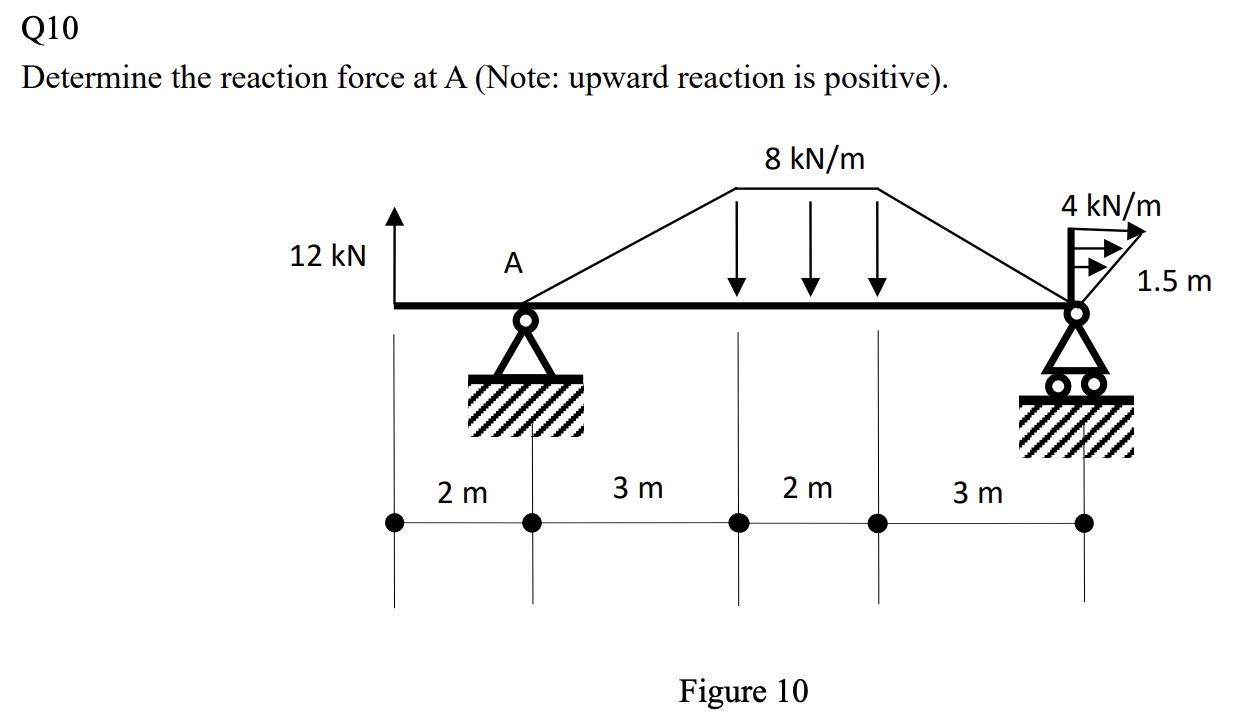
\includegraphics[width=0.8\textwidth]{img/2-8.jpg}
\end{center}
Consider units in $kN$, moment about roller:
\begin{align*}
    F_{Ax}=\frac{4\times1.5}{2}=3\ kN                                                                                                            \\
    (\frac{2}{3}\cdot 1.5\times\frac{1}{2}\cdot 4\cdot 1.5) + (8\cdot F_{Ay}) + (12\cdot 10) & = (\frac{8\cdot 3}{2}\times(6+2)+8\cdot 2\times4) \\
    F_{Ay}                                                                                   & = 4.625\ kN                                       \\
    F_A = \sqrt{3^2+4.625^2}                                                                 & = 5.513\ kN                                       \\
\end{align*}


\end{document}